\begin{problem}
Find the best approximation from the space of polynomials of degree at
most one to $f(x) = x^2 , x \in [0 , 1]$ in:
\begin{enumerate}
\item $\infty$-norm.
\item 2-norm.
\item 1-norm.
\end{enumerate}
\end{problem}

\begin{solution}
  \begin{enumerate}
  \item [{\bf $\infty$-norm: }]
    $\frac{\partial (kx + m - x^2)}{\partial x} = 0$ gives a critical
    point at $x = \frac{k}{2}$. This means the only three points we
    have to worry about is $x = 0, k/2, 1$ as they are the only
    possible maxima. The maximum error will be the smallest when all
    three maxima are equal. We used this same reasoning in the
    argument for the position of the Chebyshev points.

    If we make this demand and set the difference between the
    approximation function and $x^2$ to be equal to $\gamma$ at these
    three points we get a system of equations containing three
    equations and three unknowns.
    \begin{align}
      k \times 0  + m  - 0^2  = -\gamma \label{eq:start}\\
      k \times \frac{k}{2}  + m - \left(\frac{k}{2}\right)^2  = \gamma
      \label{eq:middle}\\
      k \times 1  + m  - 1^2   = -\gamma \label{eq:end}
    \end{align}
    Equation \ref{eq:start} gives $m = - \gamma$ and equation
    \ref{eq:middle} $k = \sqrt{8\gamma}$. Inserting this into equation
    \ref{eq:end} gives $\gamma = \frac{1}{8}$. Thus we have that the
    best approximation to $x^2$ in the approximation set of linear
    functions using the $\infty$-norm is $x - \frac{1}{8}$.
    
  \item[{\bf 2-norm: }] We want to find the best approximation to the
    function $f(x) = x^2$ by a polynomial of degree at most one
    (i.e. of the form $p(x) = ax+b$). By definition the best
    approximation minimizes the norm of the difference, that is:
    \begin{equation*}
      \min \lVert x^2-ax-b \rVert_2
    \end{equation*}
    Let us define $g(x) = x^2-ax-b$. We want to find the parameters
    $a, b$ such that the integral is minimal (note that we take the
    norm squared):
    \begin{equation*}
      \int_0^1 g(x)^2 \, dx = \frac{1}{5} - \frac{a}{2} - \frac{2b+a^2}{3} + ab + b
    \end{equation*}
    Now we take the partial derivatives of this expression with
    respect to $a$ and $b$ and make them equal to zero, obtaining $a =
    -\frac{1}{3}, b = \frac{5}{18}$. Therefore the best approximation
    polynomial is $p(x)=-\frac{1}{3}x + \frac{5}{18}$.
    
  \item [{\bf 1-norm: }] We tried to take the same approach as for the
    two norm, that is, taking the integral:
    \begin{equation*}
      \int_0^1 \lvert x^2-ax-b \rvert \, dx
    \end{equation*}
    But since we have an absolute value, we have to split the integral
    into parts. Assuming that the polynomial crosses the function
    twice (we determine this experimentally) we end up having to
    solve:
    \begin{equation*}
      \int_0^1 \lvert x^2-ax-b \rvert \, dx = \int_0^{x_1} (-x^2+ax+b)
      \, dx + \int_{x_1}^{x_2} (x^2-ax-b) \, dx+ \int_{x_2}^1
      (-x^2+ax+b) \, dx
    \end{equation*}
    Whereas it is possible to find expressions for $x_1$ and $x_2$, we
    find that the result of the integrals that we end up with is
    extremely hard to manipulate. Therefore we made a simulation in
    GeoGebra and the best possible polynomial we could find was
    $0.95x-0.15$ with $\lVert x^2-ax-b \rVert_1 = 0.06$

    It is also interesting to note that as seen on the Figure, our
    guess for the 1-norm (red) is smaller than the $\infty$-norm's
    best approximation (blue).
\begin{figure}[h]
\centering
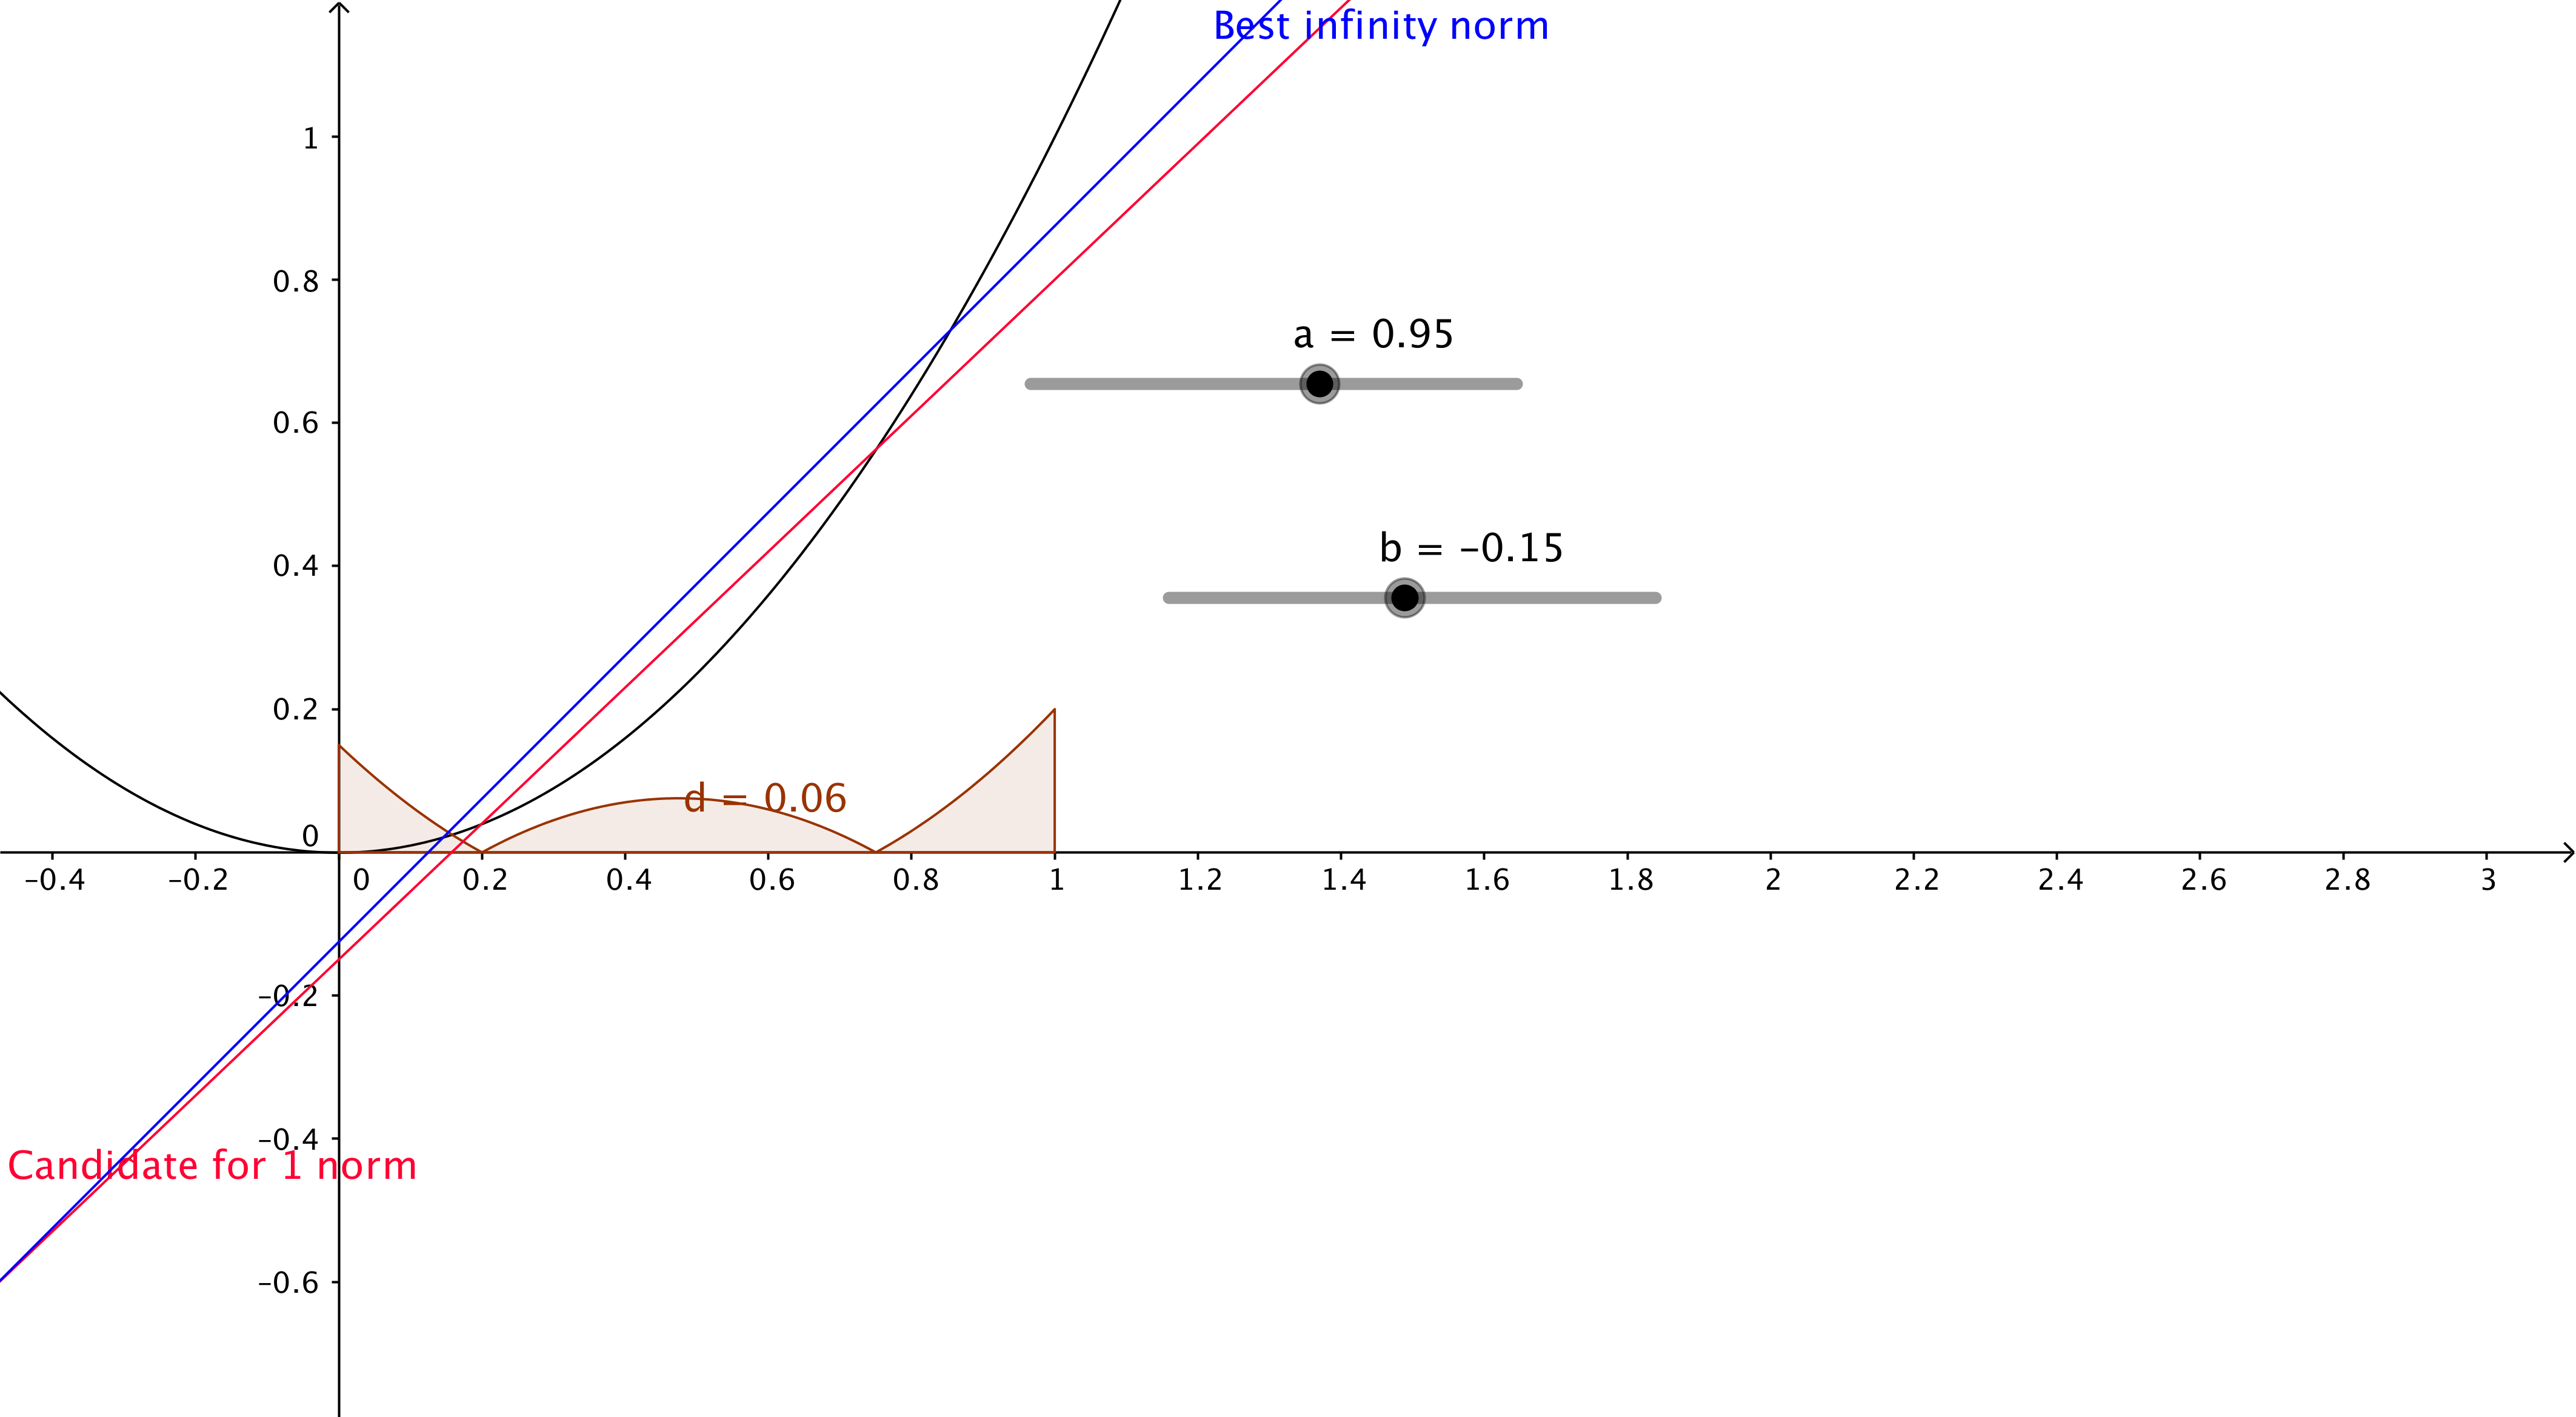
\includegraphics[scale=0.25]{task7.png}
\label{cranknic}
\end{figure}

\end{enumerate}
\end{solution}

 	

%%% Local Variables:
%%% TeX-master: "report.tex"
%%% End:
